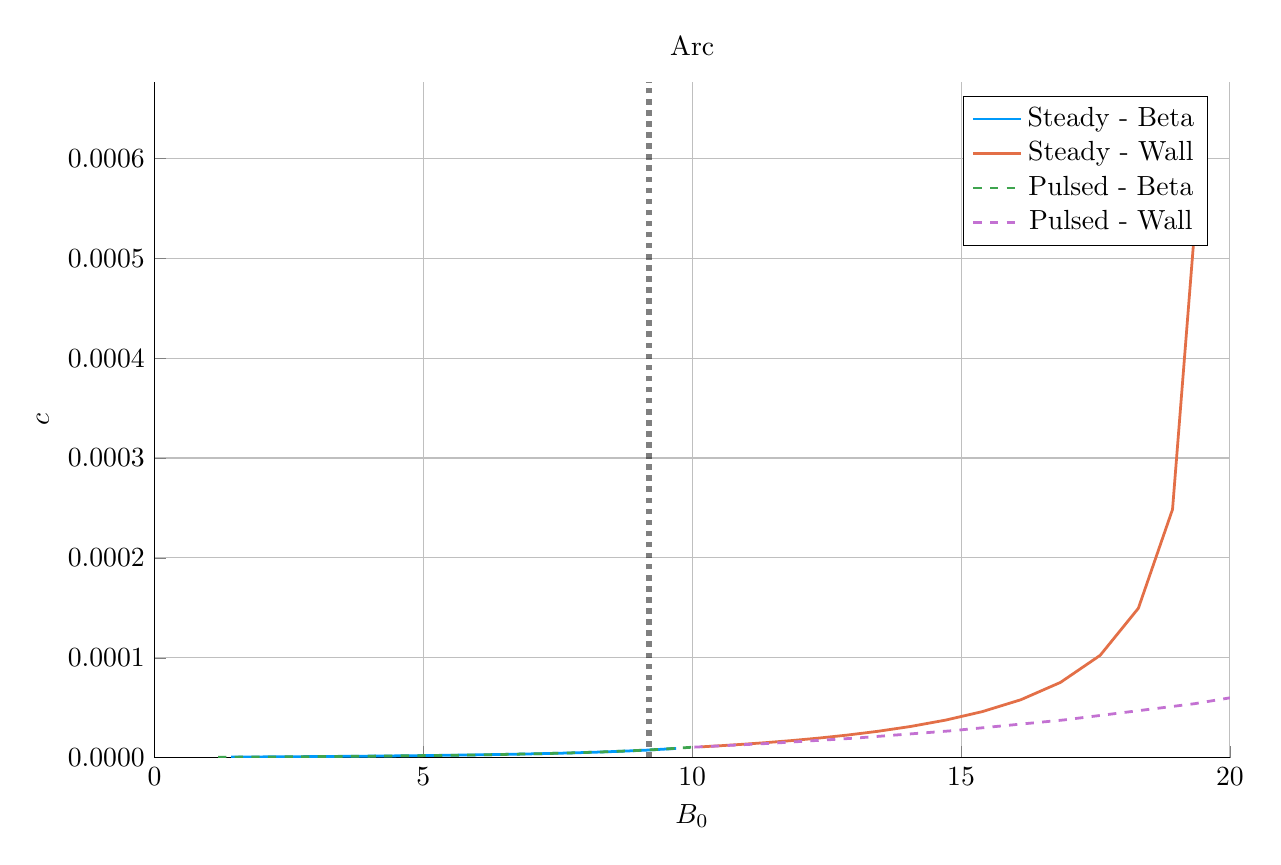
\begin{tikzpicture}[]
\begin{axis}[height = {101.6mm}, ylabel = {${c}$}, title = {Arc}, xmin = {0.0}, xmax = {20.0}, ymax = {0.0006763322696000717}, xlabel = {${B}_{0}$}, {unbounded coords=jump, scaled x ticks = false, xticklabel style={rotate = 0}, xmajorgrids = true, xtick = {0.0,5.0,10.0,15.0,20.0}, xticklabels = {0,5,10,15,20}, xtick align = inside, axis lines* = left, scaled y ticks = false, yticklabel style={rotate = 0}, ymajorgrids = true, ytick = {0.0,0.0001,0.0002,0.00030000000000000003,0.0004,0.0005,0.0006000000000000001}, yticklabels = {0.0000,0.0001,0.0002,0.0003,0.0004,0.0005,0.0006}, ytick align = inside, axis lines* = left,     xshift = 0.0mm,
    yshift = 0.0mm,
    axis background/.style={fill={rgb,1:red,1.00000000;green,1.00000000;blue,1.00000000}}
, colorbar style={title=}}, ymin = {0.0}, width = {152.4mm}]\addplot+ [color = {rgb,1:red,0.00000000;green,0.60560316;blue,0.97868012},
draw opacity=1.0,
line width=1,
solid,mark = none,
mark size = 2.0,
mark options = {
    color = {rgb,1:red,0.00000000;green,0.00000000;blue,0.00000000}, draw opacity = 1.0,
    fill = {rgb,1:red,0.00000000;green,0.60560316;blue,0.97868012}, fill opacity = 1.0,
    line width = 1,
    rotate = 0,
    solid
}]coordinates {
(9.701206080853105, 9.233893442054222e-6)
(9.162315904693079, 7.581924024905241e-6)
(8.664301107137337, 6.391914160097445e-6)
(8.203576462497304, 5.498708331860283e-6)
(7.776718537485166, 4.8065271381919635e-6)
(7.380720231870917, 4.256450195371137e-6)
(7.012886014999712, 3.81027848205469e-6)
(6.670795005901889, 3.4422087283644767e-6)
(6.352268997292712, 3.1342109140653977e-6)
(6.055344682097163, 2.8733240092172265e-6)
(5.778249464564785, 2.65000340759482e-6)
(5.519380338856715, 2.4570730234738233e-6)
(5.2772854007125325, 2.2890393764788008e-6)
(5.050647625972996, 2.141630066612971e-6)
(4.838270606140816, 2.0114756316044435e-6)
(4.639065978019038, 1.8958855025900762e-6)
(4.4520423235376105, 1.792687193705049e-6)
(4.276295348572609, 1.7001088927388161e-6)
(4.110999177018484, 1.6166924118396799e-6)
(3.9553986195015125, 1.5412277435299111e-6)
(3.8088022956698633, 1.4727032333879242e-6)
(3.6705765055641186, 1.4102672023075326e-6)
(3.54013975965751, 1.353198073116177e-6)
(3.4169578891619192, 1.3008808898982119e-6)
(3.30053966845824, 1.2527886959169922e-6)
(3.1904328903033052, 1.2084676419563948e-6)
(3.086220842019516, 1.1675249860065904e-6)
(2.9875191373772063, 1.129619353664803e-6)
(2.8939728644914635, 1.0944527806385875e-6)
(2.8052540149097247, 1.06176417079176e-6)
(2.7210591632720242, 1.0313238865928735e-6)
(2.6411073705789065, 1.0029292515129181e-6)
(2.565138287279709, 9.764007914388815e-7)
(2.492910435164382, 9.51579078490645e-7)
(2.4241996494611984, 9.28322068605278e-7)
(2.3587976646588236, 9.065028459600697e-7)
(2.296510829425685, 8.860077042652094e-7)
(2.237158937627476, 8.667345082938363e-7)
(2.180574163874242, 8.485912895699776e-7)
(2.126600093288366, 8.314950385337365e-7)
(2.075090836295778, 8.1537066222515e-7)
(2.0259102202234582, 8.001500819360802e-7)
(1.978931050353818, 7.857714496525332e-7)
(1.9340344338545452, 7.721784656626412e-7)
(1.8911091606836798, 7.593197826052489e-7)
(1.8500511361739687, 7.471484836108255e-7)
(1.8107628605384507, 7.356216241430451e-7)
(1.773152951016952, 7.246998287657966e-7)
(1.7371357028100902, 7.143469354017714e-7)
(1.7026306853269466, 7.045296807649235e-7)
(1.6695623706125668, 6.952174215819017e-7)
(1.6378597911249178, 6.863818869992876e-7)
(1.607456224302725, 6.779969582307985e-7)
(1.5782889016090462, 6.700384720530235e-7)
(1.5502987399539199, 6.624840452273636e-7)
(1.5234300935954943, 6.553129173237039e-7)
(1.4976305247952577, 6.485058097598704e-7)
(1.4728505916614916, 6.420447991596079e-7)
(1.4490436517578602, 6.359132033787388e-7)
(1.4261656801829077, 6.300954787608988e-7)
};
\addlegendentry{Steady - Beta}
\addplot+ [color = {rgb,1:red,0.88887350;green,0.43564919;blue,0.27812294},
draw opacity=1.0,
line width=1,
solid,mark = none,
mark size = 2.0,
mark options = {
    color = {rgb,1:red,0.00000000;green,0.00000000;blue,0.00000000}, draw opacity = 1.0,
    fill = {rgb,1:red,0.88887350;green,0.43564919;blue,0.27812294}, fill opacity = 1.0,
    line width = 1,
    rotate = 0,
    solid
}]coordinates {
(19.394007482712425, 0.0005636102246667265)
(18.932196567189358, 0.0002485707885891112)
(18.296989378345195, 0.00014961490155687278)
(17.587029315408756, 0.0001024837665155273)
(16.847882407994106, 7.535455397767349e-5)
(16.111374502564406, 5.800644119911708e-5)
(15.396027314547156, 4.6132319644637403e-5)
(14.710952688793137, 3.760001082585041e-5)
(14.06168447794857, 3.1248266437711164e-5)
(13.450465418483889, 2.6387573376425945e-5)
(12.877644538645335, 2.2584706344031868e-5)
(12.342394470642008, 1.9554675841374245e-5)
(11.843182246608265, 1.7102988605933875e-5)
(11.376441269625893, 1.5088134802643437e-5)
(10.944966372727551, 1.3425662493504989e-5)
(10.541663878705513, 1.2028741111849741e-5)
(10.165908182236457, 1.0847355970303777e-5)
};
\addlegendentry{Steady - Wall}
\addplot+ [color = {rgb,1:red,0.24222430;green,0.64327509;blue,0.30444865},
draw opacity=1.0,
line width=1,
dashed,mark = none,
mark size = 2.0,
mark options = {
    color = {rgb,1:red,0.00000000;green,0.00000000;blue,0.00000000}, draw opacity = 1.0,
    fill = {rgb,1:red,0.24222430;green,0.64327509;blue,0.30444865}, fill opacity = 1.0,
    line width = 1,
    rotate = 0,
    solid
}]coordinates {
(9.980483622051658, 1.0408570069232424e-5)
(9.392786903460065, 8.320194052882241e-6)
(8.79273598103983, 6.733929086567093e-6)
(8.23820290909994, 5.599667755327165e-6)
(7.725182218401588, 4.7532035261516205e-6)
(7.250078106370205, 4.1005537051689105e-6)
(6.80965553466646, 3.5842117322179836e-6)
(6.400998063035608, 3.1671013865172105e-6)
(6.0214713600430425, 2.824291394316954e-6)
(5.668691517461799, 2.5384272382325025e-6)
(5.340497445229901, 2.297074073878495e-6)
(5.034926745580058, 2.0911008589939924e-6)
(4.750194564008521, 1.913659930384533e-6)
(4.484674995755211, 1.7595214170212516e-6)
(4.236884692979903, 1.6246267337560347e-6)
(4.00546837264544, 1.5057815771973881e-6)
(3.7891859704718387, 1.400440193749856e-6)
(3.5869012239550364, 1.3065508175168696e-6)
(3.3975714987448393, 1.2224429930955414e-6)
(3.2202386987489797, 1.146744136325882e-6)
(3.0540211220494466, 1.0783168627628255e-6)
(2.8981061427709687, 1.016211301621588e-6)
(2.7517436139566023, 9.59628378533556e-7)
(2.6142398986781377, 9.078912318854637e-7)
(2.4849524463010138, 8.604227315159362e-7)
(2.363284838174807, 8.167276241161721e-7)
(2.248682232019848, 7.763782188654018e-7)
(2.140627136740878, 7.390028026862424e-7)
(2.038635448877246, 7.042761718319744e-7)
(1.9422526775794744, 6.719118083699608e-7)
(1.8510502754751532, 6.416553317887354e-7)
(1.7646219756564088, 6.132789273615371e-7)
(1.6825800061969869, 5.86576499990846e-7)
(1.6045510059627948, 5.613593275360305e-7)
(1.53017138625397, 5.374519898270995e-7)
(1.4590817483192686, 5.146883220556018e-7)
(1.3909197311384796, 4.929070678922974e-7)
(1.3253102336217724, 4.719467531580903e-7)
(1.261851128383913, 4.5163898675614897e-7)
(1.20009089049112, 4.31798738099473e-7)
(1.1394908096975784, 4.122086717244005e-7)
};
\addlegendentry{Pulsed - Beta}
\addplot+ [color = {rgb,1:red,0.76444018;green,0.44411178;blue,0.82429754},
draw opacity=1.0,
line width=1,
dashed,mark = none,
mark size = 2.0,
mark options = {
    color = {rgb,1:red,0.00000000;green,0.00000000;blue,0.00000000}, draw opacity = 1.0,
    fill = {rgb,1:red,0.76444018;green,0.44411178;blue,0.82429754}, fill opacity = 1.0,
    line width = 1,
    rotate = 0,
    solid
}]coordinates {
(29.27715761652869, 0.000188752801108687)
(25.4410619834368, 0.00011965577349061087)
(22.158819835998365, 7.917427114525168e-5)
(19.342453256965573, 5.406152685004715e-5)
(16.919364280634177, 3.7821637391118336e-5)
(14.829378672669455, 2.6981171341850862e-5)
(13.022412368922526, 1.9560831961223565e-5)
(11.456617692058645, 1.4376440771903774e-5)
(10.096901921254785, 1.0691737401461344e-5)
(9.980483622051658, 1.0408570069232424e-5)
};
\addlegendentry{Pulsed - Wall}
\addplot+ [color = {rgb,1:red,0.00000000;green,0.00000000;blue,0.00000000},
draw opacity=0.5,
line width=2,
dotted,mark = none,
mark size = 2.0,
mark options = {
    color = {rgb,1:red,0.00000000;green,0.00000000;blue,0.00000000}, draw opacity = 0.5,
    fill = {rgb,1:red,0.00000000;green,0.00000000;blue,0.00000000}, fill opacity = 0.5,
    line width = 1,
    rotate = 0,
    solid
},forget plot]coordinates {
(0.0, NaN)
(20.0, NaN)
};
\addplot+ [color = {rgb,1:red,0.00000000;green,0.00000000;blue,0.00000000},
draw opacity=0.5,
line width=2,
dotted,mark = none,
mark size = 2.0,
mark options = {
    color = {rgb,1:red,0.00000000;green,0.00000000;blue,0.00000000}, draw opacity = 0.5,
    fill = {rgb,1:red,0.00000000;green,0.00000000;blue,0.00000000}, fill opacity = 0.5,
    line width = 1,
    rotate = 0,
    solid
},forget plot]coordinates {
(9.2, 0.0)
(9.2, 0.0006763322696000717)
};
\addplot+[draw=none, color = {rgb,1:red,0.00000000;green,0.00000000;blue,0.00000000},
draw opacity=0.5,
line width=0,
solid,mark = *,
mark size = 2.0,
mark options = {
    color = {rgb,1:red,0.00000000;green,0.00000000;blue,0.00000000}, draw opacity = 0.5,
    fill = {rgb,1:red,0.00000000;green,0.00000000;blue,0.00000000}, fill opacity = 0.5,
    line width = 1,
    rotate = 0,
    solid
},forget plot] coordinates {
(9.2, NaN)
};
\end{axis}

\end{tikzpicture}
